% A LaTeX template for MSc Thesis submissions to 
% Politecnico di Milano (PoliMi) - School of Industrial and Information Engineering
%
% S. Bonetti, A. Gruttadauria, G. Mescolini, A. Zingaro
% e-mail: template-tesi-ingind@polimi.it
%
% Last Revision: October 2021
%
% Copyright 2021 Politecnico di Milano, Italy. NC-BY

\documentclass{Configuration_Files/PoliMi3i_thesis}

%------------------------------------------------------------------------------
%	REQUIRED PACKAGES AND  CONFIGURATIONS
%------------------------------------------------------------------------------

% CONFIGURATIONS
\usepackage{parskip} % For paragraph layout
\usepackage{setspace} % For using single or double spacing
\usepackage{emptypage} % To insert empty pages
\usepackage{multicol} % To write in multiple columns (executive summary)
\setlength\columnsep{15pt} % Column separation in executive summary
\setlength\parindent{0pt} % Indentation
\raggedbottom  

% PACKAGES FOR TITLES
\usepackage{titlesec}
% \titlespacing{\section}{left spacing}{before spacing}{after spacing}
\titlespacing{\section}{0pt}{3.3ex}{2ex}
\titlespacing{\subsection}{0pt}{3.3ex}{1.65ex}
\titlespacing{\subsubsection}{0pt}{3.3ex}{1ex}
\usepackage{color}

% PACKAGES FOR LANGUAGE AND FONT
\usepackage[english]{babel} % The document is in English  
\usepackage[utf8]{inputenc} % UTF8 encoding
\usepackage[T1]{fontenc} % Font encoding
\usepackage[11pt]{moresize} % Big fonts

% PACKAGES FOR IMAGES
\usepackage{graphicx}
\usepackage{transparent} % Enables transparent images
\usepackage{eso-pic} % For the background picture on the title page
\usepackage{subfig} % Numbered and caption subfigures using \subfloat.
\usepackage{tikz} % A package for high-quality hand-made figures.
\usetikzlibrary{}
\graphicspath{{./Images/}} % Directory of the images
\usepackage{caption} % Coloured captions
\usepackage{xcolor} % Coloured captions
\usepackage{amsthm,thmtools,xcolor} % Coloured "Theorem"
\usepackage{float}

% STANDARD MATH PACKAGES
\usepackage{amsmath}
\usepackage{amsthm}
\usepackage{amssymb}
\usepackage{amsfonts}
\usepackage{bm}
\usepackage[overload]{empheq} % For braced-style systems of equations.
\usepackage{fix-cm} % To override original LaTeX restrictions on sizes

% PACKAGES FOR TABLES
\usepackage{tabularx}
\usepackage{longtable} % Tables that can span several pages
\usepackage{colortbl}

% PACKAGES FOR ALGORITHMS (PSEUDO-CODE)
\usepackage{algorithm}
\usepackage{algorithmic}

% PACKAGES FOR REFERENCES & BIBLIOGRAPHY
\usepackage[colorlinks=true,linkcolor=black,anchorcolor=black,citecolor=black,filecolor=black,menucolor=black,runcolor=black,urlcolor=black]{hyperref} % Adds clickable links at references
\usepackage{cleveref}
\usepackage[square, numbers, sort&compress]{natbib} % Square brackets, citing references with numbers, citations sorted by appearance in the text and compressed
\bibliographystyle{abbrvnat} % You may use a different style adapted to your field

% OTHER PACKAGES
\usepackage{pdfpages} % To include a pdf file
\usepackage{afterpage}
\usepackage{lipsum} % DUMMY PACKAGE
\usepackage{fancyhdr} % For the headers
\fancyhf{}

% Input of configuration file. Do not change config.tex file unless you really know what you are doing. 
\input{Configuration_Files/config}

%----------------------------------------------------------------------------
%	NEW COMMANDS DEFINED
%----------------------------------------------------------------------------

% EXAMPLES OF NEW COMMANDS
\newcommand{\bea}{\begin{eqnarray}} % Shortcut for equation arrays
\newcommand{\eea}{\end{eqnarray}}
\newcommand{\e}[1]{\times 10^{#1}}  % Powers of 10 notation

%----------------------------------------------------------------------------
%	ADD YOUR PACKAGES (be careful of package interaction)
%----------------------------------------------------------------------------

%----------------------------------------------------------------------------
%	ADD YOUR DEFINITIONS AND COMMANDS (be careful of existing commands)
%----------------------------------------------------------------------------

%----------------------------------------------------------------------------
%	BEGIN OF YOUR DOCUMENT
%----------------------------------------------------------------------------

\begin{document}

\fancypagestyle{plain}{%
\fancyhf{} % Clear all header and footer fields
\fancyhead[RO,RE]{\thepage} %RO=right odd, RE=right even
\renewcommand{\headrulewidth}{0pt}
\renewcommand{\footrulewidth}{0pt}}

%----------------------------------------------------------------------------
%	TITLE PAGE
%----------------------------------------------------------------------------

\pagestyle{empty} % No page numbers
\frontmatter % Use roman page numbering style (i, ii, iii, iv...) for the preamble pages

\puttitle{
	title= Parametric machines: towards a formalization of neural networks, % Title of the thesis
	name=Martina Garavaglia, % Author Name and Surname
	course=Mathematical Engineering - Ingegneria Matematica, % Study Programme (in Italian)
	ID  = 967257,  % Student ID number (numero di matricola)
	advisor= Prof. Piercesare Secchi, % Supervisor name
	coadvisor={Mattia G. Bergomi, Pietro Vertechi}, % Co-Supervisor name, remove this line if there is none
	academicyear={2021-22},  % Academic Year
} % These info will be put into your Title page 

%----------------------------------------------------------------------------
%	PREAMBLE PAGES: ABSTRACT (inglese e italiano), EXECUTIVE SUMMARY
%----------------------------------------------------------------------------
\startpreamble
\setcounter{page}{1} % Set page counter to 1

% ABSTRACT IN ENGLISH
\chapter*{Abstract} 

\textbf{Keywords:} here, the keywords, of your thesis % Keywords

% ABSTRACT IN ITALIAN
\chapter*{Abstract in lingua italiana}
Qui va l'Abstract in lingua italiana della tesi seguito dalla lista di parole chiave.
\\
\\
\textbf{Parole chiave:} qui, vanno, le parole chiave, della tesi % Keywords (italian)

%----------------------------------------------------------------------------
%	LIST OF CONTENTS/FIGURES/TABLES/SYMBOLS
%----------------------------------------------------------------------------

% TABLE OF CONTENTS
\thispagestyle{empty}
\tableofcontents % Table of contents 
\thispagestyle{empty}
\cleardoublepage

%-------------------------------------------------------------------------
%	THESIS MAIN TEXT
%-------------------------------------------------------------------------
% In the main text of your thesis you can write the chapters in two different ways:
%
%(1) As presented in this template you can write:
%    \chapter{Title of the chapter}
%    *body of the chapter*
%
%(2) You can write your chapter in a separated .tex file and then include it in the main file with the following command:
%    \chapter{Title of the chapter}
%    \input{chapter_file.tex}
%
% Especially for long thesis, we recommend you the second option.

\addtocontents{toc}{\vspace{2em}} % Add a gap in the Contents, for aesthetics
\mainmatter % Begin numeric (1,2,3...) page numbering

% --------------------------------------------------------------------------
% NUMBERED CHAPTERS % Regular chapters following
% --------------------------------------------------------------------------
\chapter*{Introduction}
QUI L'INTRODUZIONE GENERALE AL LAVORO
The aim of this project is to establish a unified framework for deep learning in which neural networks are defined in terms of unique layer, that we call \textbf{parametric machine}.
... articolo parametric machines

%\chapter{Julia: an efficient programming language}
%\section{Introduction to Julia}
\label{sec:Introduction_to_Julia}
The programming language chosen to pursue this thesis project is Julia. Right now, Julia is a language that is little known in the data science world but brings with it great benefits both in terms of performance and usability: it is a flexible dynamic language, appropriate for scientific and numerical computing, with performance comparable to traditional statically-typed languages.  

The most significant departures of Julia from typical dynamic languages are:
\begin{enumerate}
    \item The core language imposes very little; Julia Base and the standard library are written in Julia itself, including primitive operations like integer arithmetic;
    \item A rich language of types for constructing and describing objects, that can also optionally be used to make \textbf{type declarations};
    \item The ability to define function behavior across many combinations of argument types via \textbf{multiple dispatch};
    \item Automatic generation of efficient, specialized code for different argument types;
    \item \textbf{Good performance}, approaching that of statically-compiled languages like C;
    \item Julia is an \textbf{open source project}, with all code hosted on github and several community projects underway.
\end{enumerate}


\section{Julia vs Python}
Using Julia as the programming language for this project is not a random choice: the high performance and the possibility that this language allows us to explore are many compares to other languages. 

A brief comparison between Julia and the probably better known language Python can help us understand this choice.
In terms of \textbf{speed}, Julia is much faster than Python (its execution speed is very close to that of C). From a \textbf{community} point of view, Python has been around from ages and it has a very large community of programmers in the network, so it becomes much easier to get your problems resolve online. Moreover, Julia codes can easily be made converting to or Python codes, whereas Python does not. The \textbf{libraries} in Python are in advance level and there are plenty of it, but in Julia can interfere with libraries of C and Fortran to handle with the tasks that are not already implemented. The last point regards the type of language: Julia is \textbf{dynamically typed} and you can developed code without specifying the type of object you are using, but (as we have already pointed out) the types declaration is one of the things that makes Julia very efficient. Python is also dynamically typed but it doesn't provide the benefits of types declaration.

The following table summarises the reasons why we should decide to use one language rather than the other:
\\
\begin{table}[H]
\centering 
    \begin{tabular}{|p{10em} c c|}
    \hline
    \rowcolor{bluepoli!40}
     & \textbf{Julia} & \textbf{Python} \T\B \\
    \hline \hline
    \textbf{Speed} & \checkmark & \T\B\\
    \hline
    \textbf{Community} &  & \checkmark \T\B\\
    \hline
    \textbf{Code conversion} & \checkmark &  \T\B\\
    \hline
     \textbf{Libraries} &  & \checkmark  \T\B\\
    \hline
    \textbf{Dynamically typed} & \checkmark & \checkmark \B\\
    \hline
    \end{tabular}
    \\[20pt]
    \caption{Julia vs Python: a simple comparison}
    \label{table:JuliavsPython}
\end{table}


%\chapter{A brief introduction to deep learning}
%We are going to make a short introduction to what neural networks and deep learning are, with particular reference to networks architectures we are going to exploit in the next chapters.

The primary objective of deep learning methods is to find a function that maps an input to an output in an "optimal" way (i.e., minimizing some cost function). Deep learning methods are particularly useful when the structure of the optimal solution is not known, but there is an ample dataset of "correct" examples.

The strategy to solve them is always the same: 
\begin{enumerate}
    \item Choose a differentiable parametric function $\hat{y} = f(x,p)$, where $x$ is the input and $p$ the parameters;
    \item Define a differentiable loss function $L(\hat{y})$ and minimize it with respect to $p$ (using its derivatives);
    \item Compute derivatives of $L$ with respect to $p$ and use them to find optimal parameters.
\end{enumerate}

The choice of the function $f$ is the difficult point and a fundamental goal of this work. There are different architectures we can use to develop a good model:
\begin{itemize}
    \item Dense neural networks (multilayer perceptron);
    \item Convolutional neural networks;
    \item Recurrent neural networks.
\end{itemize}

\section{Dense neural networks (multilayer perceptron)}
Dense Neural Network (DNN), which is the simplest neural network architecture, is a biologically inspired computational model. Its layers are densely connected, which means each neuron in a layer receives an input from all the neurons in the previous layer (i.e., each neuron is connected to all neurons of the previous layer) and similarly, it is an input for all the neurons in the following layers, as we can see in Figure~\ref{fig:DNN}.

\begin{figure}[H]
    \centering
    \includegraphics[width=0.6\textwidth]{Images/DNN.png}
    \caption{Dense neural network}
    \label{fig:DNN}
\end{figure}


\section{Convolutional neural networks}
A dense architecture is really simple to understand, but it ignore the structure of the problem at hand. The knowledge about the structure of natural images suggests two key principles to prevent the explosion in the number of parameters:
\begin{enumerate}
    \item \textbf{Locality:} each pixel should only received inputs from nearby pixels;
    \item \textbf{Equivariance:} a shift in the input image should correspond to a shift in the output image.
\end{enumerate}


The convolution formula with input channels $C_1$ and output channels $C_2$ is:
\begin{equation}
    J[i_1,i_2,c_2] = \sum_{c_1 \in C_1}\sum_{k_1 \in K_1}\sum_{k_2 \in K_2}{W[k_1, k_2, c_1, c_2]I[i_1 - k_1, i_2 - k_2, c_1]}
\end{equation}


\begin{figure}[H]
    \centering
    \includegraphics[width=0.7\textwidth]{Images/CNN_filter.png}
    \caption{Convolutional neural network}
    \label{fig:CNN_filter}
\end{figure}


\section{Recurrent neural networks}
Recurrent neural networks (RNN) was developed to work with sequential data. Data are sequential when their underlying temporal dynamics is more relevant than the information carried by each individual data point. 

The idea under RNN is to add knowledge of the immediate past to the current state of the network allowing output from some nodes to affect subsequent input to the same nodes (graphically, connections between nodes can create a cycle).

\begin{figure}[H]
    \centering
    \includegraphics[width=0.7\textwidth]{Images/RNN.png}
    \caption{Recurrent neural network}
    \label{fig:RNN}
\end{figure}



%\chapter{Parametric machines}
%\section{Mathematical framework}

We start by setting the mathematical framework for the study of machines. We firstly remember two key notions for deep learning: \textbf{linearity} and \textbf{differentiability}. In order to retain this concepts, we will work with normed vector spaces and Fréchet derivatives (more details in appendix \ref{appendix:a}).


\subsection{Machines}
The intuition behind parametric machines is that neural network can be considered as an endofunction $f : X \to X $ on a space of global functions $X$ (defined on all neurons on all layers). 

In a classical deep learning framework, different layers in a neural network are combined using composition. A sequence of layers
\begin{equation}
    X_0 \xrightarrow{l_1} X_1 \xrightarrow{l_2} ... \xrightarrow{l_{d-1}} X_{d-1} \xrightarrow{l_d} X_d
\end{equation}
is composed into a map $X_0 \to X_d$, and we denote the composition of functions as:
\begin{equation}
    l_dl_{d-1}...l_2l_1 : X_0 \to X_d
\end{equation}

However, we are going to consider a different framework: we consider a global space $X = \bigoplus_{i=0}^{d} X_i $ and the global endofunction:

\begin{equation}
    f = \sum_{i=1}^d l_i \in C^1(X,X)
\end{equation}

In order to establish a relation between the composition of functions and the sum of functions we consider that the output space of the network is the entire $X$ and not only the last layer space $X_d$. 


\chapter{Background}
\section{A brief introduction to artificial neural networks and deep learning}

We are going to make a short introduction to what neural networks and deep learning are, with particular reference to networks architectures we are going to exploit in the next chapters.

The primary objective of deep learning methods is to find a function that maps an input to an output in an "optimal" way (i.e., minimizing some cost function). Deep learning methods are particularly useful when the structure of the optimal solution is not known, but there is an ample dataset of "correct" examples.

The strategy to solve them is always the same: 
\begin{enumerate}
    \item Choose a differentiable parametric function $\hat{y} = f(x,p)$, where $x$ is the input and $p$ the parameters;
    \item Define a differentiable loss function $L(\hat{y})$ and minimize it with respect to $p$ (using its derivatives);
    \item Compute derivatives of $L$ with respect to $p$ and use them to find optimal parameters.
\end{enumerate}

The choice of the function $f$ is the difficult point and a fundamental goal of this work. 
There are different architectures we can use to develop a good model:
\begin{itemize}
    \item Dense neural networks (multilayer perceptron);
    \item Convolutional neural networks;
    \item Recurrent neural networks.
\end{itemize}

\subsection{Dense neural networks (multilayer perceptron)}
Dense Neural Network (DNN), which is the simplest neural network architecture, is a biologically inspired computational model \cite{DNNandCNN}. Its layers are densely connected, which means each neuron in a layer receives an input from all the neurons in the previous layer (i.e., each neuron is connected to all neurons of the previous layer) and similarly, it is an input for all the neurons in the following layers, as we can see in Figure~\ref{fig:DNN}.


\tikzset{%
  every neuron/.style={
    circle,
    draw,
    minimum size=1cm
  },
  neuron missing/.style={
    draw=none, 
    scale=4,
    text height=0.333cm,
    execute at begin node=\color{black}$\vdots$
  },
}

\begin{figure}[H]
\centering
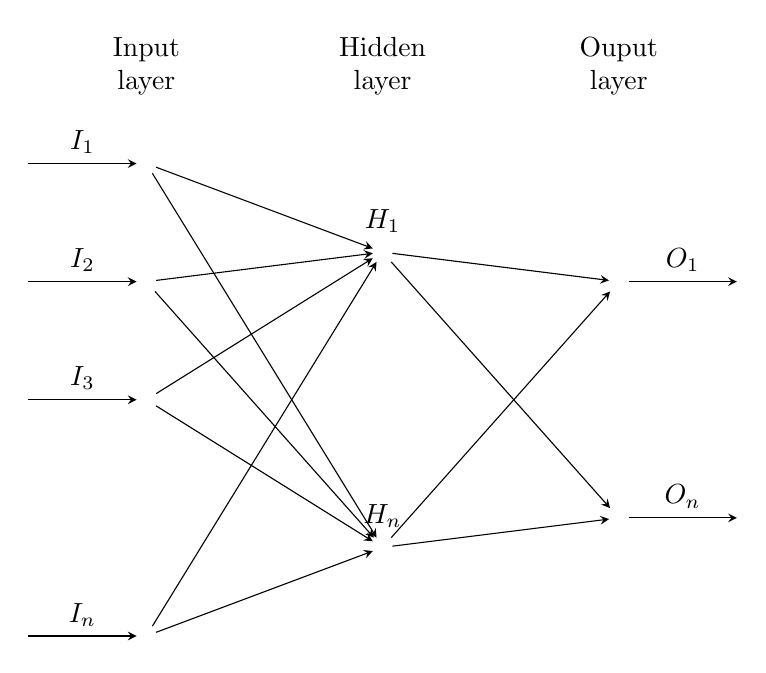
\begin{tikzpicture}[x=1.5cm, y=1.5cm, >=stealth]

\foreach \m/\l [count=\y] in {1,2,3,missing,4}
  \node [every neuron/.try, neuron \m/.try] (input-\m) at (0,2.5-\y) {};

\foreach \m [count=\y] in {1,missing,2}
  \node [every neuron/.try, neuron \m/.try ] (hidden-\m) at (2,2-\y*1.25) {};

\foreach \m [count=\y] in {1,missing,2}
  \node [every neuron/.try, neuron \m/.try ] (output-\m) at (4,1.5-\y) {};

\foreach \l [count=\i] in {1,2,3,n}
  \draw [<-] (input-\i) -- ++(-1,0)
    node [above, midway] {$I_\l$};

\foreach \l [count=\i] in {1,n}
  \node [above] at (hidden-\i.north) {$H_\l$};

\foreach \l [count=\i] in {1,n}
  \draw [->] (output-\i) -- ++(1,0)
    node [above, midway] {$O_\l$};

\foreach \i in {1,...,4}
  \foreach \j in {1,...,2}
    \draw [->] (input-\i) -- (hidden-\j);
\foreach \i in {1,...,2}
  \foreach \j in {1,...,2}
    \draw [->] (hidden-\i) -- (output-\j);

\foreach \l [count=\x from 0] in {Input, Hidden, Ouput}
  \node [align=center, above] at (\x*2,2) {\l \\ layer};
    
\end{tikzpicture}

    \caption{Dense neural network}
    \label{fig:DNN}
\end{figure}


\subsection{Convolutional neural networks}
A DNN is really simple to understand, but it ignore the structure of the problem at hand. The knowledge about the structure of natural images suggests two key principles to prevent the explosion in the number of parameters:
\begin{enumerate}
    \item \textbf{Locality:} each pixel should only received inputs from nearby pixels;
    \item \textbf{Equivariance:} a shift in the input image should correspond to a shift in the output image.
\end{enumerate}


The convolution formula with input channels $C_1$ and output channels $C_2$ is:
\begin{equation}
    J[i_1,i_2,c_2] = \sum_{c_1 \in C_1}\sum_{k_1 \in K_1}\sum_{k_2 \in K_2}{W[k_1, k_2, c_1, c_2]I[i_1 - k_1, i_2 - k_2, c_1]}
\end{equation}

In the past, DNN models were employed for image recognition. However, the full connectivity between nodes caused the
curse of dimensionality, whereas a convolutional neural netowrk (CNN) could substantially decrease the number of parameters due to
having a weight sharing structure and pooling methods
and therefore, outperform DNNs in analysing visionary
images (and not only). It is important to note that CNN is spatially
invariance, which means it does not encode the position
and orientation of object.



\begin{figure}[t!]
	\centering
	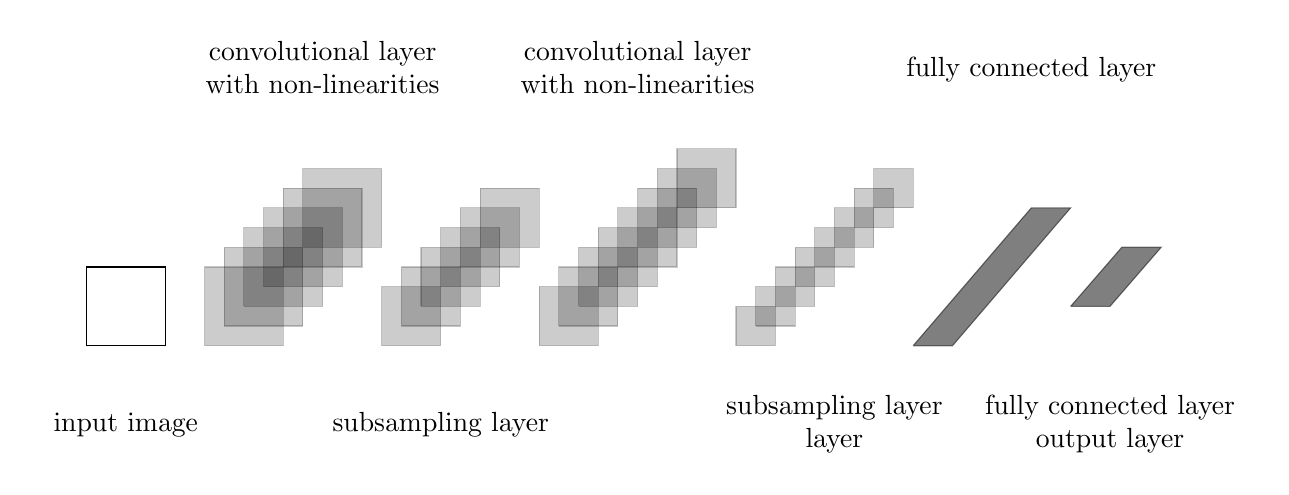
\begin{tikzpicture}
		\node at (0.5,-1){\begin{tabular}{c}input image\end{tabular}};
		
		\draw (0,0) -- (1,0) -- (1,1) -- (0,1) -- (0,0);
		
		\node at (3,3.5){\begin{tabular}{c}convolutional layer\\with non-linearities\end{tabular}};
		
		\draw[fill=black,opacity=0.2,draw=black] (2.75,1.25) -- (3.75,1.25) -- (3.75,2.25) -- (2.75,2.25) -- (2.75,1.25);
		\draw[fill=black,opacity=0.2,draw=black] (2.5,1) -- (3.5,1) -- (3.5,2) -- (2.5,2) -- (2.5,1);
		\draw[fill=black,opacity=0.2,draw=black] (2.25,0.75) -- (3.25,0.75) -- (3.25,1.75) -- (2.25,1.75) -- (2.25,0.75);
		\draw[fill=black,opacity=0.2,draw=black] (2,0.5) -- (3,0.5) -- (3,1.5) -- (2,1.5) -- (2,0.5);
		\draw[fill=black,opacity=0.2,draw=black] (1.75,0.25) -- (2.75,0.25) -- (2.75,1.25) -- (1.75,1.25) -- (1.75,0.25);
		\draw[fill=black,opacity=0.2,draw=black] (1.5,0) -- (2.5,0) -- (2.5,1) -- (1.5,1) -- (1.5,0);
		
		\node at (4.5,-1){\begin{tabular}{c}subsampling layer\end{tabular}};
		
		\draw[fill=black,opacity=0.2,draw=black] (5,1.25) -- (5.75,1.25) -- (5.75,2) -- (5,2) -- (5,1.25);
		\draw[fill=black,opacity=0.2,draw=black] (4.75,1) -- (5.5,1) -- (5.5,1.75) -- (4.75,1.75) -- (4.75,1);
		\draw[fill=black,opacity=0.2,draw=black] (4.5,0.75) -- (5.25,0.75) -- (5.25,1.5) -- (4.5,1.5) -- (4.5,0.75);
		\draw[fill=black,opacity=0.2,draw=black] (4.25,0.5) -- (5,0.5) -- (5,1.25) -- (4.25,1.25) -- (4.25,0.5);
		\draw[fill=black,opacity=0.2,draw=black] (4,0.25) -- (4.75,0.25) -- (4.75,1) -- (4,1) -- (4,0.25);
		\draw[fill=black,opacity=0.2,draw=black] (3.75,0) -- (4.5,0) -- (4.5,0.75) -- (3.75,0.75) -- (3.75,0);
		
		\node at (7,3.5){\begin{tabular}{c}convolutional layer\\with non-linearities\end{tabular}};
		
		\draw[fill=black,opacity=0.2,draw=black] (7.5,1.75) -- (8.25,1.75) -- (8.25,2.5) -- (7.5,2.5) -- (7.5,1.75);
		\draw[fill=black,opacity=0.2,draw=black] (7.25,1.5) -- (8,1.5) -- (8,2.25) -- (7.25,2.25) -- (7.25,1.5);
		\draw[fill=black,opacity=0.2,draw=black] (7,1.25) -- (7.75,1.25) -- (7.75,2) -- (7,2) -- (7,1.25);
		\draw[fill=black,opacity=0.2,draw=black] (6.75,1) -- (7.5,1) -- (7.5,1.75) -- (6.75,1.75) -- (6.75,1);
		\draw[fill=black,opacity=0.2,draw=black] (6.5,0.75) -- (7.25,0.75) -- (7.25,1.5) -- (6.5,1.5) -- (6.5,0.75);
		\draw[fill=black,opacity=0.2,draw=black] (6.25,0.5) -- (7,0.5) -- (7,1.25) -- (6.25,1.25) -- (6.25,0.5);
		\draw[fill=black,opacity=0.2,draw=black] (6,0.25) -- (6.75,0.25) -- (6.75,1) -- (6,1) -- (6,0.25);
		\draw[fill=black,opacity=0.2,draw=black] (5.75,0) -- (6.5,0) -- (6.5,0.75) -- (5.75,0.75) -- (5.75,0);
		
		\node at (9.5,-1){\begin{tabular}{c}subsampling layer\\layer\end{tabular}};
		
		\draw[fill=black,opacity=0.2,draw=black] (10,1.75) -- (10.5,1.75) -- (10.5,2.25) -- (10,2.25) -- (10,1.75);
		\draw[fill=black,opacity=0.2,draw=black] (9.75,1.5) -- (10.25,1.5) -- (10.25,2) -- (9.75,2) -- (9.75,1.5);
		\draw[fill=black,opacity=0.2,draw=black] (9.5,1.25) -- (10,1.25) -- (10,1.75) -- (9.5,1.75) -- (9.5,1.25);
		\draw[fill=black,opacity=0.2,draw=black] (9.25,1) -- (9.75,1) -- (9.75,1.5) -- (9.25,1.5) -- (9.25,1);
		\draw[fill=black,opacity=0.2,draw=black] (9,0.75) -- (9.5,0.75) -- (9.5,1.25) -- (9,1.25) -- (9,0.75);
		\draw[fill=black,opacity=0.2,draw=black] (8.75,0.5) -- (9.25,0.5) -- (9.25,1) -- (8.75,1) -- (8.75,0.5);
		\draw[fill=black,opacity=0.2,draw=black] (8.5,0.25) -- (9,0.25) -- (9,0.75) -- (8.5,0.75) -- (8.5,0.25);
		\draw[fill=black,opacity=0.2,draw=black] (8.25,0) -- (8.75,0) -- (8.75,0.5) -- (8.25,0.5) -- (8.25,0);
		
		\node at (12,3.5){\begin{tabular}{c}fully connected layer\end{tabular}};
		
		\draw[fill=black,draw=black,opacity=0.5] (10.5,0) -- (11,0) -- (12.5,1.75) -- (12,1.75) -- (10.5,0);
		
		\node at (13,-1){\begin{tabular}{c}fully connected layer\\output layer\end{tabular}};
		
		\draw[fill=black,draw=black,opacity=0.5] (12.5,0.5) -- (13,0.5) -- (13.65,1.25) -- (13.15,1.25) -- (12.5,0.5);
	\end{tikzpicture}
	\caption{Convolutional neural network}
	\label{fig:traditional-convolutional-network}
\end{figure}



\subsection{Recurrent neural networks}
Recurrent neural networks (RNN) was developed to work with sequential data. Data are sequential when their underlying temporal dynamics is more relevant than the information carried by each individual data point. 

The idea under RNN is to add knowledge of the immediate past to the current state of the network allowing output from some nodes to affect subsequent input to the same nodes (graphically, connections between nodes can create a cycle).



\begin{figure}[H]
\centering
\begin{tikzpicture}[item/.style={circle,draw,thick,align=center}, itemc/.style={item,on chain,join}]
 \begin{scope}[start chain=going right,nodes=itemc,every
 join/.style={-latex,very thick},local bounding box=chain]
 \path node (A0) {$A$} node (A1) {$A$} node (A2) {$A$} node[xshift=2em] (At)
 {$A$};
 \end{scope}
 \node[left=1em of chain,scale=2] (eq) {$=$};
 \node[left=2em of eq,item] (AL) {$A$};
 \path (AL.west) ++ (-1em,2em) coordinate (aux);
 \draw[very thick,-latex,rounded corners] (AL.east) -| ++ (1em,2em) -- (aux) 
 |- (AL.west);
 \foreach \X in {0,1,2,t} 
 {\draw[very thick,-latex] (A\X.north) -- ++ (0,2em)
 node[above,item,fill=gray!10] (h\X) {$h_\X$};
 \draw[very thick,latex-] (A\X.south) -- ++ (0,-2em)
 node[below,item,fill=gray!10] (x\X) {$x_\X$};}
 \draw[white,line width=0.8ex] (AL.north) -- ++ (0,1.9em);
 \draw[very thick,-latex] (AL.north) -- ++ (0,2em)
 node[above,item,fill=gray!10] {$h_t$};
 \draw[very thick,latex-] (AL.south) -- ++ (0,-2em)
 node[below,item,fill=gray!10] {$x_t$};
 \path (x2) -- (xt) node[midway,scale=2,font=\bfseries] {\dots};
\end{tikzpicture}
\caption{Recurrent neural network}
\label{fig:RNN}
\end{figure}

\section{Parametric machines}
The aim of this section is to establish the mathematical framework we want to use and define what parametric machines are and can be used for. For this purpose, I'll borrow extensively from the article \cite{PMachines}. Parametric machines have been studied in different mathematical framework, but we are going to use functional analysis to establish the mathematical properties.

\subsection{Machines}
We start by setting the mathematical framework for the study of machines. We firstly remember two key notions for deep learning: linearity and differentiability. In order to retain this concepts, we will work with normed vector spaces and Fréchet derivatives (more details in appendix \ref{appendix:a}).

The intuition behind parametric machines is that neural network can be considered as an endofunction $f : X \to X $ on a space of global functions $X$ (defined on all neurons on all layers). 

In a classical deep learning framework, different layers in a neural network are combined using composition. A sequence of layers
\begin{equation}
    X_0 \xrightarrow{l_1} X_1 \xrightarrow{l_2} ... \xrightarrow{l_{d-1}} X_{d-1} \xrightarrow{l_d} X_d
\end{equation}
is composed into a map $X_0 \to X_d$, and we denote the composition of functions as:
\begin{equation}
    l_dl_{d-1}...l_2l_1 : X_0 \to X_d
\end{equation}

However, this framework brings with it some disadvantages: shortcut connections are not supported and non-sequential architectures fail to be created. 


Now we are going to consider the global space $X = \bigoplus_{i=0}^{d} X_i $ and the global endofunction:

\begin{equation}
    f = \sum_{i=1}^d l_i \in C^1(X,X)
\end{equation}

In order to establish a relation between the composition of functions and the sum of functions we consider that the output space of the network is the entire $X$ and not only the last layer space $X_d$. 

Let the input function be the continuously differentiable inclusion map $g \in C^1(X_0, X)$. The map g embeds the input data into an augmented space, which encompasses input, hidden layers, and output. The network transforms the input map g into an output map $h \in C^1(X_0, X)$. From a practical perspective, h computes the activation values of all the layers and stores not only the final result, but also all the activations of the intermediate layers.
In particular, we have that $f$ (sum of all layers) and $g$ (input function) are sufficient to determine $h$ (output function).
Indeed, $h$ is the unique map in $C^1(X_0,X)$ satisfying:

\begin{equation}
    h = g + fh
    \label{machine_eq}
\end{equation}

The minimum requirement to ensure a well-defined input-output mapping is the existence of a unique solution of \ref{machine_eq} for any choice of input function $g$. Thanks to the sum-based structure of the global function, layers are no longer required to be sequential, but they must obey a weaker condition of independence (a concept that we will deepen in section TOT).

Then, we define a machine as:

\textbf{Definition 1.}  Let $X$ be a normed vector space. Let $k \in \mathbb{N} \cup {{\infty}}$. An endofunction $f \in C^k(X,X)$ is a \textit{k-differentiable machine} if, for all normed vector space $X_0$ and
for all map $g \in C^k(X_0, X)$, there exists a unique map $h \in C^k(X_0,X)$ such that eq. \ref{machine_eq} holds. We refer to $X_0$ and $X$ as input space and machine space, respectively.
We refer to eq. \ref{machine_eq} as the \textit{machine equation}.

From now on, we assume $k=1$ (machines are 1-differentiable), that allow for backpropagation, even if the results presented below can be adapted in a straightforward way to $k>1$.

Eq. \ref{machine_eq} can be reformulated as:
\begin{equation}
    (id-f)h = g
\end{equation}
and we can establish that $f$ is a machine if and only if the composition with $id-f$ induces a bijection $C^1(X_0,X) \xrightarrow{\sim} C^1(X_0,X)$ for all normed vector space $X_0$. This condition is satisfied if $id-f$ is an isomorphism:


\textbf{Proposition .1} Let $X$ be a normed vector space. $f \in C^1(X,X)$ is a \textit{machine} if and only if $id - f$ is an isomorphism. Whenever that is the case, the \textit{resolvent} of $f$ is the mapping:
\begin{equation}
    R_f = (id-f)^{-1}
\end{equation}
Then, $h = g+fh$ if and only if $h=R_fg$.

It follows that the derivative of a machine, as well as its dual, are also machines, a relevant information to perform parameter optimization.

\textbf{Proposition 2.} Let $f \in C^1(X,X)$ be a machine. Let $x_0 \in X$. Then, the derivative $Df(x_0)$, a bounded linear endofunction in $B(X,X)$, and its dual $(Df(x_0))^{*} \in B(X^*, X^*)$ are machines with resolvents:
\begin{equation*}
    R_{Df(x_0)} = DR_f(x_0) \ \ and \ \ R_{{Df(x_0)}^*} = (DR_f(x_0))^*
\end{equation*}
respectively.

\textbf{Example 1.} In order to give a practical intuition, standard sequential neural networks are machines, in fact if we consider the normed vector space $X = \bigoplus_{i=0}^{d} X_i$ and, for each $i \in {1,...,d}$ a map $l_i \in C^1(X_{i-1}, X_i)$. Let $f = \sum_{i=1}^d l_i$, the inverse of $id-f$ can be constructed explicitly via the sequence:
\begin{equation*}
    y_0 = x_0 \ \ and \ \ y_i = l_i(y_{i-1}) + x_i \ \ for i \in {1,...,d}
\end{equation*}


It satisfies:
\begin{align*}
    (y_0,...,y_d) = (x_0, l_1(y_0) + x_1, ..., l_d(y_{d-1}) + x_d) = \\(\widetilde{x_0}, l_1(y_0) + \widetilde{x_1} - l_1(\widetilde{x_0}),...,l_d(y_{d-1}) + \widetilde{x_d} - l_d(\widetilde{x}_{d-1}))
\end{align*}

By induction, $y_i = \widetilde{x_i}$ for all $i \in {0,...,d}$. Hence, the inverse of $id-f$ corresponds to:
\begin{equation*}
    R_f(x_0,...,x_d) = (y_0,...,y_d)
\end{equation*}

\textbf{Example 2.} Let us consider a bounded linear operator $f \in B(X,X)$ and $f$ be nilpotent, i.e. there exists $n \in \mathbb{N}$ such that $f^n = 0$, then $f$ is a machine and the resolvent can be constructed explicitly as

\begin{equation*}
    (id-f)^{-1} = id + f + f^2 + ... + f^{n-1}
\end{equation*}

\subsection{Depth}

The goal of this section if to discuss a common generalization of endofunctions, namely machine of \textit{finite depth}.


\chapter{Time machines}
\input{Chapters/2_time_machines.tex}

\chapter{Implementation}
implementazione delle parametric machines spiegate tramite uno pseudocodice

\chapter{A case study: }
\input{Chapters/5_case_study.tex}

\chapter{Conclusion}

%-------------------------------------------------------------------------
%	BIBLIOGRAPHY
%-------------------------------------------------------------------------

\addtocontents{toc}{\vspace{2em}} % Add a gap in the Contents, for aesthetics
\bibliography{Thesis_bibliography} % The references information are stored in the file named "Thesis_bibliography.bib"

%-------------------------------------------------------------------------
%	APPENDICES
%-------------------------------------------------------------------------

\cleardoublepage
\addtocontents{toc}{\vspace{2em}} % Add a gap in the Contents, for aesthetics
\appendix
\chapter{Fréchet derivative}
\label{appendix:a}

The Fréchet derivative is sometimes known as strong derivative and can be seen as a generalization of the gradient to arbitrary vector spaces.

Let $V$ and $W$ be normed vector spaces and $U \subseteq V$ be an open subset of $V$. A function $f: U \to W$ is called \textbf{Fréchet differentiable} at $x \in U$ if there exists a bounded linear operator $A: V \to W$ such that:
\begin{equation}
    \lim_{||h|| \to 0} \frac{||f(x + h) - f(x) - Ah||_W}{||h||_V} = 0
\end{equation}

The limit here is meant in the usual sense of a limit of a function defined on a metric space.

\chapter{Appendix B}
It may be necessary to include another appendix to better organize the presentation of supplementary material.


% LIST OF FIGURES
\listoffigures

% LIST OF TABLES
\listoftables

% LIST OF SYMBOLS
% Write out the List of Symbols in this page
\chapter*{List of Symbols} % You have to include a chapter for your list of symbols (
\begin{table}[H]
    \centering
    \begin{tabular}{lll}
        \textbf{Variable} & \textbf{Description} & \textbf{SI unit} \\\hline\\[-9px]
        $\bm{u}$ & solid displacement & m \\[2px]
        $\bm{u}_f$ & fluid displacement & m \\[2px]
    \end{tabular}
\end{table}

% ACKNOWLEDGEMENTS
\chapter*{Acknowledgements}
Here you might want to acknowledge someone.

\cleardoublepage

\end{document}
